\chapter*{Popis a rozbor problému}

\par Geoinformační systémy a jejich softwary přinášejí celou řadu funkcí pro vizualizaci, zpracování a analýzu geoprostorových dat. Jejich součástí je také spousta funkcí používaných v kartografii. Ovšem mnoho potřebných funkcí, jako je například generalizace prvků, není součástí těchto softwarů. V dnešní digitální době je ovšem i taková funkce pro kartografické práce potřebná a jelikož se v současnosti téměř veškerá činnost přesouvá do digitálního světa, objevují se pro kartografy nové výzvy v podobě řešení kartografických problémů pomocí počítačových algoritmů.

\par Každý prvek na mapě musí být zobrazen vhodnými kartografickými vyjadřovacími prostředky (bod, linie, polygon). Součástí každé mapy je měřítko. Podle určitého měřítka se zobrazují na mapě i prvky obsažené v mapě. S tím souvisí i vhodné zobrazení prvků v závislosti na měřítku. Bude –li mapa zobrazovat vesnici s přilehlými lesy a ornou půdou, nemá smysl, aby byly všechny prvky na mapě vykresleny do detailů. Čtenáře mapy bude hlavně zajímat, jaký prvek se v daném místě vyskytuje. Je tedy žádoucí jednotlivé objekty v mapě zjednodušit, ale zároveň musí platit, aby stále nesly stejnou informaci o objektu a aby generalizovaný tvar stále odpovídal danému prvku. Jinak řečeno, podle Monmoniera (2018) dobrá mapa čtenáři do jisté míry lže (potlačuje pravdu) proto, aby mohl vidět, co potřebuje.

\par Generalizovat se tedy mohou liniové a polygonové prvky. Tato úloha se zabývá generalizací polygonů, konkrétně generalizací budov pomocí tzv. \emph{konvexní obálky} a \emph{min-max boxu} (dále jen \emph{MMB}), též označovaného jako \emph{bounding box}.
\bigbreak

\section*{Konvexní obálka}

\par Je dána konečná množina $n$ bodů $S = [p_1, p_2, ..., p_n]$ v $\mathbb{R}^2$, kde $p_i = [x_i, y_i]$. Podle Bayera (2023a) je konvexní obálka (v angličtině \emph{convex hull}) $\mathcal{H}$ nejmenší konvexní mnohoúhelník $P$ obsahující $S$ (a tedy neexistuje vlastní podmnožina $P' \subset P$, která splňuje tuto definici). Další definice konvexní obálky jsou uvedeny následovně:

\begin{enumerate}
  \item Konvexní obálka $\mathcal{H}$ konečné množiny $S$ představuje konvexní mnohoúhelník $P$ s nejmenší plochou.
  \item Konvexní obálka $\mathcal{H}$ konečné množiny $S$ představuje průsečnici všech polorovin obsahujících $S$.
  \item Konvexní obálka $\mathcal{H}$ konečné množiny $S$ představuje sjednocení všech trojúhelníků, jejichž vrcholy tvoří body v $S$.
\end{enumerate}

\par Podle Bayera (2023, s. 4) \emph{„množinu $S$ označíme jako konvexní, pokud spojnice libovolných dvou prvků leží zcela uvnitř této množiny“}.

\par Konvexní obálka (\emph{Obrázek 1}) se používá pro řadu algoritmů. Pomocí její konstrukce je možné rychle najít tzv. \emph{bounding box}, označován i jako \emph{min-max box} (podle Wooda (2008) takový obdélník, který je kolmý na osy souřadnicového systému \emph{x} a \emph{y} a minimálně ohraničuje složitější polygon), který představuje nejzákladnější generalizaci polygonu. Dále lze pomocí konstrukce několika konvexních obálek nad množinou bodů najít střed datasetu (Bayer 2023a), v jiných oborech nachází využití především v detekci kolizí (plánování pohybu robotů), různých statistických analýzách, analýzách tvarů objektů a pod. 

\begin{figure}[h]
\centering
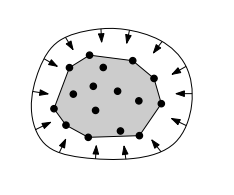
\includegraphics[width=8cm]{convexhull} 
    \caption{Ukázka konvexní obálky (převzato z de Berg a kol. (2008, s. 3)).}
\end{figure}

\par Způsobů konstrukce konvexní obálky je mnoho, v této úloze jsou konkrétně implementovány dva algoritmy: \textbf{\emph{Jarvis Scan}} a \textbf{\emph{Graham Scan}}. Některé algoritmy pro konstrukci konvexní obálky jsou také převoditelné do vyšších dimenzí než je  $\mathbb{R}^2$. V této úloze bude ovšem věnovaná pozornost čistě problémům v $\mathbb{R}^2$ prostoru.
\bigbreak

\subsection*{Jarvis Scan}

\par Tento algoritmus (označován také jako \emph{Gift Wrapping Algorithm}) je jednoduchý a snadno implementovatelný. Představuje vůbec jeden z nejpoužívanějších postupů pro tvorbu konvexní obálky v $\mathbb{R}^2$ i v $\mathbb{R}^3$. Vychází z předpokladu, že v množině bodů $S$ nejsou tři kolineární body (Bayer 2008). Je založen na principu opakovaného hledání maximálního úhlu $\omega_{max}$ mezi poslední hranou konvexní obálky $\mathcal{H}$ tvořenou body $p_{j-1}$, $p_j$ a následující hranou tvořenou body $p_j$, $p_{j+1}$. Bod $p_{j+1}$ hledáme ze všech $p_i \in S$, které dosud nejsou součástí $\mathcal{H}$. Složitost algoritmu je $O(n^2)$, nehodí se pro velké datasety (Bayer 2023a). Pro nalezení bodu $p_{j+1}$ lze nalézt i minimální úhel $\theta$ s poslední hranou (\emph{Obrázek 2}).

\begin{figure}[h]
\centering
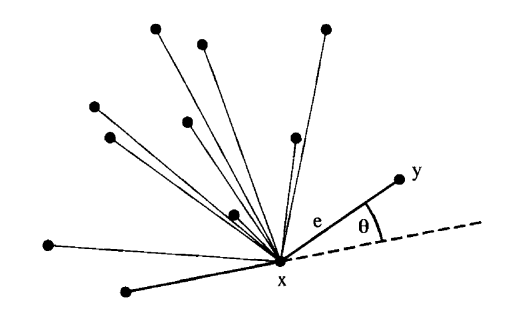
\includegraphics[width=8cm]{jarvisscan} 
    \caption{Jiný přístup ke konstrukci Jarvis Scan algoritmu. Následující hrana $e$ svírá nejmenší úhel $\theta$ s předchozí hranou (převzato z Rourke (2005, s. 69)).}
\end{figure}

\newpage

\par V prvním kroku algoritmu je nutné nalézt počáteční bod – pivota $q = [x_q, y_q]$ (časová složitost $O(n)$), který se automaticky stane součástí konvexní obálky $\mathcal{H}$:

\begin{equation*}
y_q = \underset{\forall p_i \in S}{\min}(y_i)
\end{equation*}

\par Poté se inicializuje pomocný bod $p_{j-1} = [x_{q}-1, y_q]$, pak $p_j = q$ a provede se vyhledání následujícího bodu $p_{j+1}$ nalezením úhlu $\omega_{max}$ způsobem popsaným výše.

\begin{algorithm}[h]
\caption{Jarvis Scan}\label{alg:cap}
\begin{algorithmic}
\Require $pol: polygon$
\Ensure $\mathcal{H}: {\text{\emph{konvexní obálka}}}$
\State
\State $q \gets {\text{$\underset{\forall p_i \in S}{\min}(y_i)$}}$
\State $p_{j-1} \gets {\text{inicializuj pomocný bod se souřadnicemi $[x_{q}-1, y_q]$} }$
\State $p_j \gets q$ 
\State {\text{přidej $q \to \mathcal{H}$}}
\State
\While {true}
  \State $\omega_{max} \gets 0$ \Comment{inicializuj maximální úhel}
  \State $i_{max} \gets -1$ \Comment{inicializuj index patřící bodu $p_{j+1}$}
  \State
  \For{každý bod $p_i$ z polygonu $pol$}
     \If{$p_j \neq p_i$}
      \State {\text{$\omega \gets \measuredangle{p_{j-1}, p_j, p_i}$}}
      \If{$\omega > \omega_{max}$}
      \State $\omega_{max} \gets \omega$ \Comment{aktualizuj maximální úhel}
      \State $i_{max} \gets i$ \Comment{aktualizuj index patřící bodu $p_{j+1}$}
      \EndIf
    \EndIf
  \EndFor
  \State
  \State {\text{přidej $p_{j+1}$ $\to \mathcal{H}$}}
  \State $p_{j-1} \gets p_j$
  \State $p_j \gets p_{j+1}$
  \State
  \If{$p_j = q$}
  \State {\textbf{break}} \Comment{zlom cyklus pokud je následující bod pivotem}
  \EndIf
\EndWhile
\State
\State {\text{\textbf{vrať} konvexní obálku  $\mathcal{H}$}}

\end{algorithmic}
\end{algorithm}

\newpage

\subsection*{Graham Scan}

\par Za jeden z vůbec prvních algoritmů pro nalezení konvexní obálky se považuje algoritmus popsaný Ronaldem Grahamem v roku 1972 (Rourke 2005). Tento algoritmus využívá pro tvorbu konvexní obálky kritérium pravotočivosti (resp. levotočivosti (Bayer 2023)), při kterém se posuzuje úhel  $\omega_i$ mezi dvěma úsečkami procházejícími trojici bodů: $p_{j-1}, p_j, p_{j+1}$. Uvažujme počáteční bod (pivot) $q = [x_q, y_q]$ se souřadnicemi: 

\begin{equation*}
x_q, y_q = \underset{\forall p_i \in S}{\min}(x_i, y_i)
\end{equation*}

\par Protože může existovat více bodů se stejnou hodnotou $y$, je zvykem také uvažovat s jednou z extrémních hodnot $x$ pro jednoznačné nalezení pivota.
\par Dále jsou všechny body $p_i$ setříděné vzestupně podle jejich úhlu $\omega_i$ mezi osou $x$ a spojnicí $\overline{ qp_j}$. Protože může existovat více bodů $p_i$ se stejným $\omega_i$, setříděné body se pak znovu setřídí podle jejich euklidovské vzdálenosti od $q$ (\emph{Obrázek 3}). 

\begin{figure}[h]
\centering
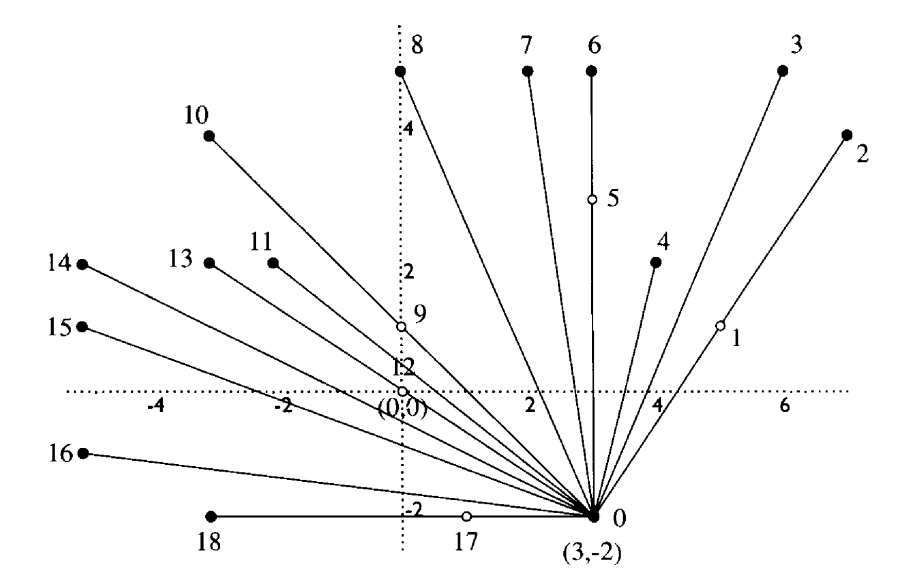
\includegraphics[width=11cm]{grahamscan} 
    \caption{Setřídění bodů $p_i$ nejprv podle $\omega_i$, pak podle jejich vzdálenosti od zvoleného $q$ (převzato z Rourke (2005, s. 76)).}
\end{figure}

\par Spojením setříděných bodů $p_i$ je pak vytvořen nekonvexní mnohoúhelník tvořen body $p_j$, který se pomocí kritéria pravotočivosti (resp. levotočivosti) provádí na konvexní mnohoúhelník (viz \emph{Obrázek 4}). Do konvexní obálky $\mathcal{H}$ se okamžitě přidají body $q$ a první setříděný bod $p_j$.

\par Kritérium levotočivosti pak determinuje příslušnost dalších bodů $p_j$ ke konvexní obálce $\mathcal{H}$ následovně:

\begin{equation*} p_j\begin{cases} \notin \mathcal{H}, & \text{$p_{j+1} \in \sigma_r(p_j, p_{j+1})$}, \\ ? \in \mathcal{H}, & \text{$p_{j+1} \in \sigma_l(p_j, p_{j+1})$}, \\\end{cases}\end{equation*}

\par kde $\sigma_r$ a $\sigma_l$ označují pravou, resp. levou polorovinu vzhledem k vektoru $\overrightarrow{p_{j-1}p_j}$.

\par V prvním případě bod $p_j$ nebude součástí konvexní obálky $\mathcal{H}$ a dále s ním nebudeme uvažovat, vrátíme se o jeden vrchol zpět ($p_j = p_{j-1}$), doplníme dvojici bodů předcházejícím a následujícím doposud nevyloučeným vrcholem a provádíme sken znova. V druhém případě bude $p_j$ možná součástí konvexní obálky. Posuneme se o jeden vrchol vpřed a zkoumáme toto kritérium u bodů $p_j, p_{j+1}, p_{j+2}$; tento postup opakujeme i pro další trojice bodů.

\par Algoritmus skončí, když $p_j = p_{n-1}$ (kde $n$ je počet vrcholů polygonu). Jeho časová složitost je $O(n\log{n})$. Ve vlastní implementaci se posuzuje pravotočivost místo levotočivosti vzhledem k orientaci souřadnicového systému.

\begin{figure}[h]
\centering
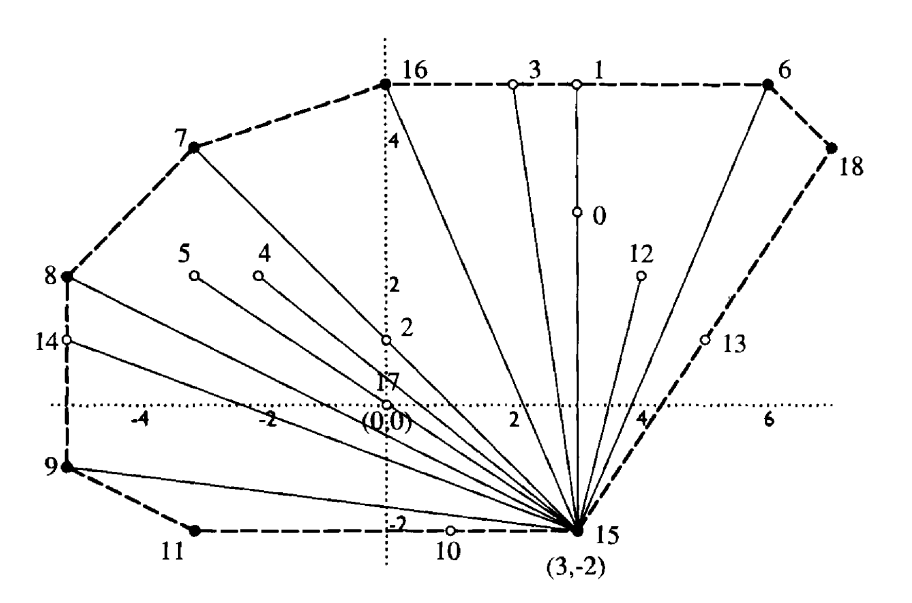
\includegraphics[width=11cm]{grahamscan2} 
    \caption{Vytvořena konvexní obálka pomocí algoritmu Graham Scan (převzato z Rourke (2005, s. 85)).}
\end{figure}

\bigbreak

\subsection*{Singulární případy}

\par U obou zmíněných algoritmů vycházíme z předpokladu, že počet vrcholů polygonu $n \geq 3$. Ve vlastní implementaci je na případ, když $n < 3$ upozorněno, a konvexní obálka nad takovým prvkem nebude vytvořena.

\bigbreak

\begin{algorithm}[h]
\caption{Graham Scan}\label{alg:cap}
\begin{algorithmic}
\Require $pol: polygon$
\Ensure $\mathcal{H}: {\text{\emph{konvexní obálka}}}$
\State $q \gets {\text{$\underset{\forall p_i \in S}{\min}(x_i, y_i)$}}$
\State seřaďBodyVPolygonu($pol, q$) \Comment pomocná funkce
\State $S \gets$ inicializuj zásobník
\State $n \gets$ počet vrcholů $pol $
\State
  \For{každý bod $p_j$ ze setříděného polygonu $pol$}
     \While{délka zásobníku $S \geq 2$}
      \If{$p_{j+1} \in \sigma_r(p_j, p_{j+1})$} \Comment{pravotočivost}
      \State {\textbf{break}} 
      \Else \Comment{levotočivost nebo kolinearita bodů}
      \State {S.pop()} \Comment{vyjmi $p_j$ ze zásobníku}
      \EndIf
    \EndWhile
    \State {\text{přidej $p_{j+1}$ $\to \mathcal{H}$}}
  \EndFor
\State {\text{\textbf{vrať} konvexní obálku  $\mathcal{H}$}}

\end{algorithmic}
\end{algorithm}

\bigbreak

\section*{Detekce hlavních směrů budov}

\par V rámci generalizace budovy je nutné najít její hlavní směry pro zachování orientace původního nezgeneralizovaného objektu a návaznosti na ostatní prvky v mapě. Není například žádoucí, aby generalizovaná budova vbíhala za uliční, či říční linie. Je důležité, aby výsledný zjednodušený tvar budovy byl vhodně natočen vzhledem k respektování polohy ostatních prvků v mapě. Existuje několik algoritmů pro nalezení hlavních směrů budovy:

\begin{itemize}
    
    \item \emph{Minimum Area Enclosing Rectangle},
    \item \emph{Wall Average},
    \item \emph{Longest Edge},
    \item \emph{Weighted Bisector}.
\end{itemize}

\bigbreak

\subsection*{Minimum Area Enclosing Rectangle Algorithm}

\par Principem algoritmu \emph{Minimum Area Enclosing Rectangle} (dále jen \emph{MAER}) je nalézt takový obdélník, jehož plocha bude minimální. Jinde je tento algoritmus znám pod názvem \emph{Minimum-Area Bounding Rectangle}. Na podobném principu pracuje i algoritmus \emph{Rotating Calipers}.

\par Je dána množina $n$ bodů $S$ v $\mathbb{R}^2$. Výstupem je takový obdélník $\mathcal{R}$, který opíše množinu $S$. Obdélník $\mathcal{R}$ nelze zkonstruovat napřímo. Proto je potřebné množinu $S$ předzpracovat do konvexní obálky $\mathcal{H}$. Výsledný $\mathcal{R}$ má pak alespoň jednu hranu kolineární s hranou konvexní obálky $\mathcal{H}$ (Bayer 2023a).

\par Hlavní myšlenkou tohoto algoritmu je (v momentě, kdy je zkonstruována konvexní obálka tvořena \emph{n} body) procházet všechny hrany konvexní obálky a pro každou její hranu nalézt MMB, jehož hrana je rovnoběžná s právě procházenou hranou konvexní obálky (viz \emph{Obrázek 5}). Ze všech \emph{n} obdélníků se vybere ten s minimální plochou. Během chodu algoritmu je tedy nutné uchovávat informaci o nejmenší možné ploše a zároveň si k této ploše pamatovat hranu, jež je kolineární s hranou minimálního opsaného obdélníku (Eberley 2020).

\par Algoritmus pak bude probíhat následovně: Během procházení každé hrany v konvexní obálce se vypočte úhel směrnice $\sigma$ příslušné hrany. Pak se konvexní obálka $\mathcal{H}$ otočí o příslušný úhel $\sigma$ a zkonstruuje se pro ni MMB. Pokud plocha nového MMB bude menší než dosud nejmenší spočtená plocha, pak se tento MMB a jeho příslušný úhel zapamatují (Bayer 2023a).

\begin{figure}[h]
\centering
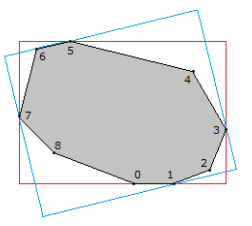
\includegraphics[width=7cm]{koliner_edge.png} 
    \caption{Ukázka zkonstruování min-max boxu, který je rovnoběžný s hranou konvexní obálky tvořenou body 5 a 6. (převzato z Eberley (2020, s. 4)).}
\end{figure}
\newpage

\begin{algorithm}[h]
\caption{Minimum Area Enclosing Rectangle}\label{alg:cap}
\begin{algorithmic}
\Require $pol: polygon$
\Ensure $\mathcal{R}: polygon$
\State
\State $\mathcal{H} \gets {\text{vytvoř konvexní obálku}}$
\State $R \gets {\text{první opsaný obdélník}}$ 
\State $A \gets {\text{spočti iniciální plochu }}\mathcal{R}$
\State $sigma\_min \gets 0$ \Comment{inicializuj úhel}
\State
\For{každou hranu $edge$ z konvexní obálky $\mathcal{H}$}
    \State pro $edge$ spočti směrnici $sigma$
    \State natoč $\mathcal{H}$ o úhel $-sigma$
    \State zkonstruuj nový obdélník $\mathcal{R}'$ a spočti novou plochu $A'$
    \State
    \If{$A' < A$} \Comment{nová minimální plocha}
    \State  $A'$ se stává nejmenší nalezenou plochou $A$
    \State zapamatuj si hodnoty $\mathcal{R} = \mathcal{R}'$ a $sigma\_min = sigma$
    \EndIf
\EndFor
\State
\State {\text{\textbf{vrať} nejmenší $\mathcal{R}$ natočený o příslušnou hodnotu $sigma\_min$}}

\end{algorithmic}
\end{algorithm}

\bigbreak
\bigbreak
\subsection*{Wall Average Algorithm}

\par Tento algoritmus patří k více komplexnějším. Základním principem je pro každou hranu v polygonu spočítat poměr

\begin{equation}\biggl\lfloor \frac{\Delta\sigma_i}{\frac{\pi}{2}} \biggr\rfloor,\end{equation}

\par kde $\Delta \sigma_i$ je rozdíl úhlů $\sigma_i$ a $\sigma{'}$, $\sigma_i$ je směrnice právě zpracované hrany polygonu a $\sigma{'}$ představuje jednu libovolně zvolenou směrnici jedné z hran polygonu.

\par Pro každou hranu polygonu tvořeného $n$ body se vypočte směrnice $\sigma_i$. Dále se vybere libovolná hrana s úhlem $\sigma'$, o níž se otočí polygon. Poté se pro každou hranu spočte rozdíl 

\begin{equation} \Delta\sigma_i = \sigma_i - \sigma'. \end{equation}

\par Pro jasnější představu je přiložen \emph{Obrázek 6}, který vlevo ukazuje vypočtené směrnice $\sigma_i$ a vpravo rozdíl úhlů  $\Delta\sigma_i$ (Bayer 2023a).

\begin{figure}[h]
\centering
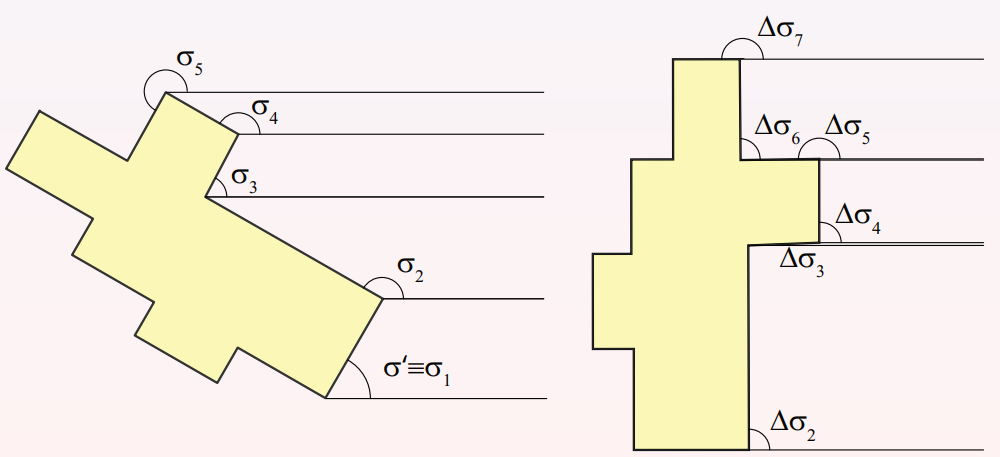
\includegraphics[width=14cm]{images/Wall_average.png} 
    \caption{Metoda Wall average: vpravo: směrnice $\sigma_i$ spočtená pro každou hranu, vlevo: rozdíl $\Delta\sigma_i$ (převzato z Bayer (2023a s. 40).}
\end{figure}

\newpage

\par Následně pro každou hodnotu $\Delta\sigma_i$ spočteme (1), čímž se získá zaokrouhlený podíl $k_i$:

\begin{equation}k_i = \biggl\lfloor \frac{\Delta\sigma_i}{\frac{\pi}{2}} \biggr\rfloor.\end{equation}

\par Po vypočtení $k_i$ je pak potřebné vypočítat zbytky $r_i$ a odchylky od $0 \pm k\pi$, respektive  $\frac{\pi}{2} \pm k\pi$:

\begin{equation} r_i = \Delta\sigma_i - k_i \frac{\pi}{2} .\end{equation}

\par Hlavní směr budovy natočení je pak dán vztahem:

\begin{equation} \sigma = \sigma' + \sum_{i=1}^n \frac{r_i \cdot s_i}{s_i}, \end{equation}

\par kde $s_i$ je délka hrany $i$. V rámci vlastní implementace je používán aritmetický průměr místo váženého průměru. 

\begin{algorithm}[h]
\caption{Wall Average Algorithm}\label{alg:cap}
\begin{algorithmic}
\Require $pol: polygon$
\Ensure $\mathcal{R}: polygon$
\State
\State $\sigma' \gets {\text{spočítej směrnici první hrany polygonu }} pol$
\State $r\_aver \gets 0$ \Comment{inicializuj průměrný zbytek}
\State
\For{každou hranu $edge$ v polygonu $pol$}
    \State pro $edge$ spočti směrnici $\sigma_i$
    \State $\Delta\sigma_i \gets $spočti rozdíl $\sigma_i - \sigma'$
    \State
    \If{$\Delta\sigma_i < 0$} \Comment{korekce úhlu $\Delta\sigma_i$ }
    \State k úhlu $\Delta\sigma_i$ přičti periodu $2\pi$
    \EndIf
    \State
    \State vypočti koeficient $k_i$ a výsledek zaokrouhli
    \State vypočti zbytek $r_i$ pro aktuální iteraci
    \State aktualizuj průměrný zbytek $r\_aver$ o hodnotu $r_i$
\EndFor
\State
\State vypočti průměrný zbytek pro polygon $r\_aver$
\State nastav průměrný úhel $\sigma\_aver$ $=$ $\sigma'$ + $r\_aver$
\State $\mathcal{R} \gets {\text{vytvoř obdélník kolem }} r\_aver$ 
\State 
\State {\text{\textbf{vrať} $\mathcal{R}$ }}

\end{algorithmic}
\end{algorithm}

\newpage

\subsection*{Longest Edge Algorithm}

\par Tento jednoduchý algoritmus předpokládá, že hlavní směr polygonu (budovy) je jeho nejdelší hrana. Druhý hlavní směr je pak kolmý na nejdelší hranu. Podél nejdelší strany budovy pak bude natočen výsledný obdélník, jehož delší strana bude rovnoběžná s nejdelší hranou. \emph{Obrázek 7} ilustruje princip algoritmu. Zelený obdélník je rovnoběžný s nejdelší hranou polygonu (Bayer 2023a).

\begin{figure}[h]
\centering
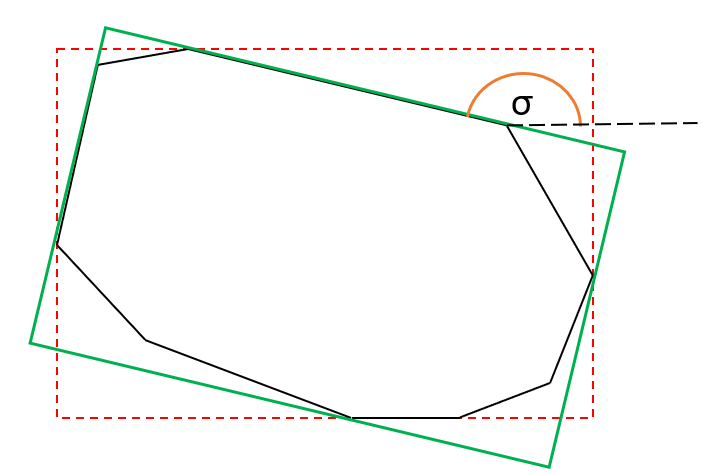
\includegraphics[width=8cm]{images/longest_edge.png}
    \caption{Opsaný obdélník podél nejdelší hrany polygonu natočený o úhel $\sigma$ (vlastní zpracování).}
\end{figure}

\par Pro danou množinu $S$, jejíž hranice tvoří $n$ bodů v $\mathbb{R}^2$ je hledána nejdelší hrana polygonu, podél které se zkonstruuje MMB. Výstupem algoritmu je opsaný obdélník $\mathcal{R}$ kolem množiny $S$ rovnoběžný s nejdelší hranou polygonu.

\begin{algorithm}[h]
\caption{Longest Edge Algorithm}\label{alg:cap}
\begin{algorithmic}
\Require $pol: polygon$
\Ensure $\mathcal{R}: polygon$
\State
\State $longest\_edge \gets -1$ \Comment{inicializuj nejdelší hranu}
\State
\For{každou hranu $edge$ v polygonu}
    \State pro $edge$ spočti její délku $dist$
    \State
    \If{$dist > longest\_edge$} \Comment{nová nejdelší hrana}
    \State  $edge$ s délkou $dist$ se stává nejdelší hranou v polygonu
    \State pro tuto $edge$ vypočti její směrnici $\sigma$
    \EndIf
\EndFor
\State
\State $rotate\_pol \gets {\text{rotuj polygon o }}- \sigma$ 
\State $\mathcal{R} \gets {\text{vytvoř obdélník kolem }} rotate\_pol$ 
\State
\State {\text{\textbf{vrať} $\mathcal{R}$ }}

\end{algorithmic}
\end{algorithm}
\newpage

\bigbreak

\subsection*{Weighted Bisector Algorithm}

\par Tento algoritmus pro detekci hlavních směrů použije dvě nejdelší vnitřní úhlopříčky nalezené v polygonu. Jde tedy o nalezení takových úhlopříček, které neprotínají žádnou z hran polygonu. Pro test, zda nalezená úhlopříčka protíná hranu polygonu, se použije opakovaná aplikace Halfplane testu (Bayer 2023a).

\par Mějme úsečku $\overline{\rm P_1P_2}$ tvořenou body $P_1 = [x_1, y_1]$ a $P2 = [x_2, y_2]$ a úsečku $\overline{\rm P_3P_4}$ tvořenou body \newline $P3 = [x_3, y_3]$ a $P4 = [x_4, y_4]$. 
\par Pro tyto body se provede 4x analýza koncového bodu úsečky vzhledem ke druhé úsečce a naopak. Jedná se o výpočet determinantu (Bayer 2023b).

\begin{equation} 
\begin{aligned}
            t_1 = \begin{vmatrix} x_2 - x_1 & y_2 - y_1 \\ x_4 - x_1 & y_4 - y_1  \end{vmatrix} &&
            t_2 = \begin{vmatrix} x_2 - x_1 & y_2 - y_1 \\ x_3 - x_1 & y_3 - y_1  \end{vmatrix} \\
            t_3 = \begin{vmatrix} x_4 - x_3 & y_4 - y_3 \\ x_1 - x_3 & y_1 - y_3  \end{vmatrix} &&
            t_4 = \begin{vmatrix} x_4 - x_3 & y_4 - y_3 \\ x_2 - x_3 & y_2 - y_3 \end{vmatrix}
\end{aligned}
\end{equation}

\par Pokud $t_1$ a $t_2$ mají stejné znaménko, nebo $t_3$ a $t_4$ mají stejné znaménko, pak mezi úsečkami $\overline{\rm P_1P_2}$ a $\overline{\rm P_3P_4}$ neexistuje průsečík. Bude-li mít $t_1$ a $t_2$ stejné znaménko, pak se koncové body úsečky nacházejí ve stejné polorovině vůči druhé úsečce (2023b).

\par Po nalezení dvou nejdelších úhlopříček se spočte pro každou úhlopříčku jejich délka ($s_1$ a $s_2$) a směrnice ($\sigma_1$ a $\sigma_2$). Hlavní směr budovy $\sigma$ se pak vypočte pomocí vztahu:

\begin{equation} 
    \sigma = \frac{s_1\sigma_1 + s_2\sigma_2}{s_1 + s_2}
\end{equation} 

\newpage

\begin{algorithm}[h]
\caption{Weighted Bisector Algorithm}\label{alg:cap}
\begin{algorithmic}
\Require $pol: polygon$
\Ensure $\mathcal{R}: polygon$
\State
\State zkontroluj, zda má polygon více jak 3 body \Comment{pro polygon tvořený 3 body neexistuje úhlopříčka}
\State $diagonals \gets $najdi všechny možné úhlopříčky
\State {\text{\textbf{seřaď}}} úhlopříčky podle délky 
\State inicializuj hodnoty $\sigma1$, $dist1$, $\sigma2$, $dist2$ $\gets None$
\State
\For{každou $diagonal$ z listu $diagonals$}
    \For{každou hranu $edge$ v polygonu $pol$}
        \If{$diagonal$ má průsečík s $edge$}
        \State {\text{\textbf{pokračuj}}}
        \Else \Comment{úhlopříčka nemá průsečík – jedná se o vnitřní úhlopříčku}
        \State $test$ = $True$
        \EndIf 
    \EndFor 
    \State
    \If{$test$ = $True$}
    \State {\text{\textbf{pokračuj}}} \Comment{nejde o vnitřní uhlopříčku}
    \Else
        \If {$dist1 = None$} \Comment{vypočti směrnici a délku první úhlopříčky}
        \State $\sigma1 \gets $spočti směrnici úhlopříčky $diagonal$
        \State $dist1 \gets $ vypočti délku úhlopříčky $diagonal$
        \Else \Comment{vypočti směrnici a délku druhé úhlopříčky}
        \State $\sigma2 \gets $spočti směrnici úhlopříčky $diagonal$
        \State $dist2 \gets $ vypočti dílku úhlopříčky $diagonal$
        \State {\text{\textbf{break}}}
        \EndIf
    \EndIf
\EndFor
\State
\State $\sigma \gets (dist1 * \sigma1 + dist2 * \sigma2) / (dist1 + dist2)$ \Comment{hlavní směr polygonu}
\State $rotate\_pol \gets {\text{rotuj polygon o }}- \sigma$ 
\State $\mathcal{R} \gets {\text{vytvoř obdélník kolem }} rotate\_pol$ 
\State
\State {\text{\textbf{vrať} $\mathcal{R}$ }}

\end{algorithmic}
\end{algorithm}

\par V rámci této úlohy byl pro každý algoritmus výsledný obdélník $\mathcal{R}$ zmenšen tak, aby jeho plocha odpovídala ploše původního polygonu.